% build like: latex -output-directory pdf ./outline.tex
\documentclass[onepage=true]{article}

% GraphViz Dot allows us to draw graph diagrams.
\usepackage{tikz}
\usetikzlibrary{positioning}
\usetikzlibrary{fit}

\title{What's a Kernel}
\author{Rylan Lens\_r Kellogg}

\begin{document}
\maketitle

\section{Kernel Overview}

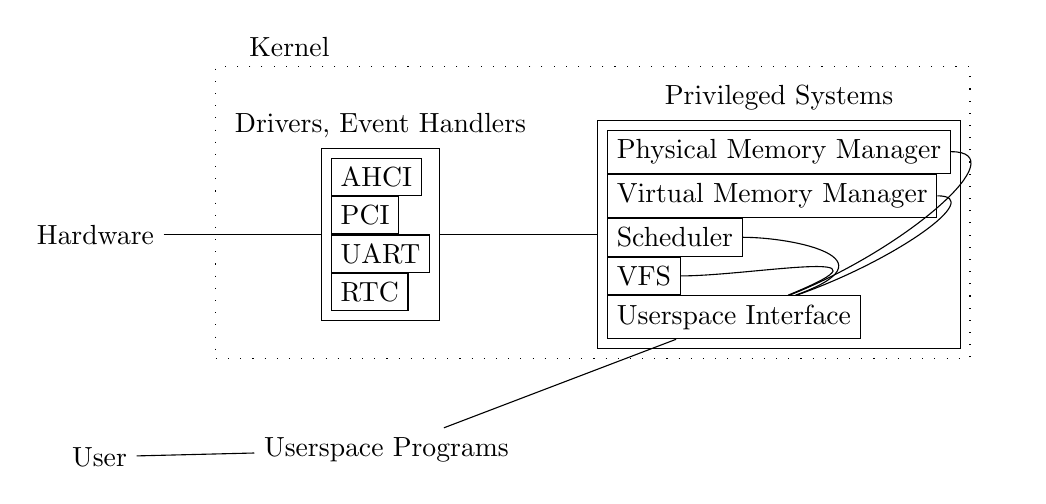
\begin{tikzpicture}[
    main/.style = {draw, circle}
  ]
  \node (hardware) {Hardware};

  \matrix[right=2cm of hardware, nodes=draw, draw=black, label={[name=drivers label] Drivers, Event Handlers}] (drivers) {
    \node (ahci) {AHCI}; \\
    \node (ahci) {PCI}; \\
    \node (uart) {UART}; \\
    \node (rtc) {RTC}; \\
  };

  \matrix[right=2cm of drivers, nodes=draw, draw=black, label={[name=privileged label] Privileged Systems}] (privileged) {
    \node (pmm) {Physical Memory Manager}; \\
    \node (vmm) {Virtual Memory Manager}; \\
    \node (sched) {Scheduler}; \\
    \node (vfs) {VFS}; \\
    \node (user interface) {Userspace Interface}; \\
  };
  \draw (user interface) to[in=east, out=north east] (pmm);
  \draw (user interface) to[in=east, out=north east] (vmm);
  \draw (user interface) to[in=east, out=north east] (sched);
  \draw (user interface) to[in=east, out=north east] (vfs);

  \node[draw,loosely dotted,fit=(drivers) (drivers label) (privileged) (privileged label),label={150:Kernel}] (kernel) {};

  \node[below left=of privileged] (user programs) {Userspace Programs};

  \node (user) [below left=of kernel] {User};

  \draw (hardware)--(drivers);
  \draw (drivers)--(privileged);
  \draw (user programs)--(user interface);
  \draw (user programs)--(user);
\end{tikzpicture}

\subsection{Hardware Drivers, Hardware Event Handlers}

Hardware works in a particular way, and most of the time software has to initialize, probe, poke, and prod hardware before it does what we want it to. Drivers are the software that directly interact with the hardware.

A lot of hardware has the ability to initiate things to happen (a keyboard's key being pressed, a timer going off, etc); hardware like this will usually use what's called a hardware interrupt. Interrupt handlers, just functions in the kernel, may be registered for specific interrupts; for example, the keyboard interrupt handler will map scancodes to the data they represent and write it to stdin of the init process for userspace processes to be able to respond to user input.

\subsection{Memory Management}

\subsubsection{Physical}
The Physical Memory Manager (often just \emph{PMM}) handles the allocation of physical pages of RAM. That is, you may lock a page or pages for use for a particular purpose, and the PMM won't give out those pages when more memory is requested, at least until the locked page or pages are freed.

\subsubsection{Virtual}
To be clear, the Virtual Memory Manager has nothing to do with the Physical Memory Manager, other than the fact that they both involve memory.

The Virtual Memory Manager (often just \emph{VMM}) handles the mapping of virtual addresses to physical addresses within page maps. With the virtual memory manager, we can sort of "trick" the computer into thinking that it is reading from an address when in reality that address is just another name for some other address; you can think of it like being able to register a URL that redirects to another.

The VMM is what allows each user process to be in it's own sandbox. We give each process a unique page map---one that maps nearly every address to an invalid address except for a few mappings, like the program's own code, the program's stack, and the program's heap---and the only possible addresses it can successfully access all originate from the program itself. As you can imagine, this makes it difficult to affect any other running process on the system.

\subsection{Scheduler}

If you can imagine, an OS that only had one process (that being the kernel process) wouldn't be that useful these days. We like to be able to run multiple processes at once: the kernel, the init process, some servers... In order to run all these different processes, we use the Scheduler.

The Scheduler is basically just a flat list of (running) processes, which keep track of things like the current working directory, allocated memory owned by the process, and more. At regular intervals (from a timer interrupt), the running process is taken over, what's called \emph{pre-empted}, by a function that sets the running process to sleeping and chooses another process from it's list to run next. To do this, it requires saving the CPU context of the process, then loading the CPU context from another.

\subsection{Virtual File System}

The VFS, as it's called. This is basically just a list of (open) files, which house things like the filepath, the drivers used to operate on the file, and more. There are also mount points, but the VFS' main job is to maintain a flat list of opened files, and provide the ability to operate on them.

\subsection{Userspace Interface}

The user owns their hardware, so, obviously, they'd like to use it. The problem is that if we just let any program do anything, it'd be way too easy to delete the kernel after visiting a website. So, each user program gets its own sandbox to play in, far removed from directly interacting with any hardware, for safety and usability. But ... if every program isn't even able to interact with the hardware, what would the computer even be able to do? Run an infinite no-op loop?

For a userspace program to interact with hardware, it must make a system call into the kernel, which has an elevated privilege level and can access any hardware it wants. This system call is just a function with a really weird way of calling it, passing arguments, and returning values, but it ultimately works just like a function.

This separation of access means that userspace programs are only allowed to do what the kernel allows them to do, when it comes to hardware. This means, with careful planning, most major problems may be avoided (i.e. a single program allocating all the available RAM, or anything to that effect).

\end{document}
